\documentclass[11pt]{article}
%Gummi|065|=)
\usepackage[utf8]{inputenc}
\title{\textbf{Diseño de un PWM apartir de amplificador y transistor}}
\author{Cabrera Gutièrrez Raùl
\\ 
Mecatrònica 4ª
\\ \textbf{Matricula: 18213157}
\\ Docente: Moran Garabito Carlos Enrique}
\date{}
\usepackage{graphicx}
\begin{document}
\begin{figure}[htp]
\centering

\includegraphics[scale=2.00]{/home/raulcb/Downloads/ed3c.jpeg}
\caption{.}
\label{.}
\end{figure}

\maketitle
\section{Diseño de un PWM}
La modulación por ancho de pulsos (también conocida como PWM, siglas en inglés de pulse-width modulation) de una señal o fuente de energía es una técnica en la que se modifica el ciclo de trabajo de una señal periódica (una senoidal o una cuadrada, por ejemplo), ya sea para transmitir información a través de un canal de comunicaciones o para controlar la cantidad de energía que se envía a una carga.
\\

El PWM es de gran ayuda en convertidores de voltaje, ya que sabemos que un amplificador operacional, es adaptado para que las ondas generadas a partir de la entrada sean mayores ya cauando van de salida, siendo esta la modulaciòn de pulso elèctrico que pueda recibir a captaciones demovimientos de la corriente que fluye y sea de mayor impulso.

\begin{figure}[htp]
\centering
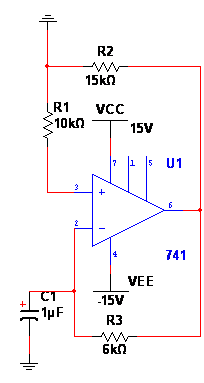
\includegraphics[scale=0.40]{/home/raulcb/Downloads/PWM.png}
\caption{.}
\label{.}
\end{figure}


\section{Construcciòn}
La construcciòn tìpica de un circuito PWM  se lleva a cabo mediante un comparador con dos entradas y una salida. Una de las entradas se conecta a un oscilador de onda,mientras que la otra queda disponible para la señal moduladora. En la salida la frecuencia es generalmente igual a la de la señal dientes de sierra y el ciclo de trabajo està en funciòn de la portadora.


\section{Desventaja}
L aprincipal desventaja que presentan los circuitos PWM es la posibilidad de que haya interferencia generada por radifrecuencia. Èstas pueden minimizarse ubicando el controlador cerca de la carga y realizando un filtrado de la fuente de alimentaciòn.

\begin{figure}[htp]
\centering
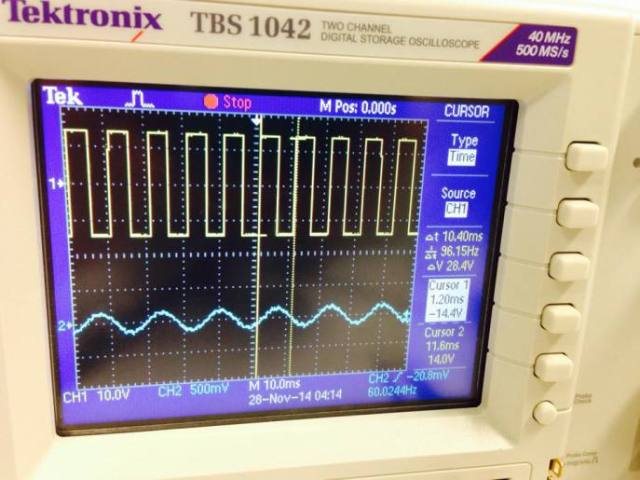
\includegraphics[scale=0.50]{/home/raulcb/Downloads/12.jpg}
\caption{.}
\label{.}
\end{figure}


\end{document}
